\begin{name}
	{\tenchude}
	{\tendethi}
	{\tentruong}
	{\thoigian}
\end{name}
\setcounter{ex}{0}\setcounter{bt}{0}
\TN
\Opensolutionfile{ans}[ans/ansDe4-TN1]
\begin{ex}%[0D1N1-1]
	Trong các câu sau, câu nào là mệnh đề?
	\choice
	{Số $\pi $ có phải là số nguyên không?}
	{\True Số $4 $ là một số nguyên tố}
	{Tam giác đều  có $3$ góc bằng nhau và bằng $60^\circ$ phải không?}
	{$a^2+b^2=c^2 $}
	\loigiai{
		\lq\lq  Số $4 $ là một số nguyên tố\rq\rq\ là một mệnh đề.
	}
\end{ex}

\begin{ex}%[0D1H1-3]
	Cho mệnh đề: \lq\lq  Có một học sinh trong lớp 10A không thích học môn Toán\rq\rq. Mệnh đề phủ định của mệnh đề này là:
	\choice
	{\True \lq\lq  Mọi học sinh trong lớp 10A đều thích học môn Toán\rq\rq}
	{\lq\lq  Mọi học sinh trong lớp 10A đều không thích học môn Toán\rq\rq}
	{\lq\lq  Mọi học sinh trong lớp 10A đều thích học môn Văn\rq\rq}
	{\lq\lq  Có một học sinh trong lớp 10A thích học môn Toán\rq\rq}
	\loigiai{
		Phủ định của mệnh đề: \lq\lq  Có một học sinh trong lớp 10A không thích học môn Toán\rq\rq là mệnh đề \lq\lq  Mọi học sinh trong lớp 10A đều thích học môn Toán\rq\rq.}
\end{ex}

\begin{ex}%[0-HK1-1819, SGD Bà Rịa - Vũng Tàu, 2018-2019]%[Phat Dang Tan]%[0D1N2-1]
	Cho tập hợp $A=\{x\in \mathbb{N}|x\leq 5\}$. Tập $A$ được viết dưới dạng liệt kê các phần tử là
	\choice
	{$A=\{1;2;3;4\}$}
	{$A=\{1;2;3;4;5\}$}
	{\True $A=\{0;1;2;3;4;5\}$}
	{$A=\{0;1;2;3;4\}$}
	\loigiai{
		$A=\{x\in \mathbb{N}\vert x\leq 5\}=\{0;1;2;3;4;5\}$.
	}
\end{ex}

\begin{ex}%[Dự án Giảng 10-11 Nhóm Toán & LaTex, Mui Doan]%[0D1H3-3]
	Cho $A=(-\infty;5]$ và $B=(0;+\infty)$. Tập hợp $A\cap B$ là
	\choice
	{\True $(0;5]$}
	{$[0;5)$}
	{$(0;5)$}
	{$(-\infty;+\infty)$}
	\loigiai
	{
		Ta có $A\cap B = (-\infty;5]\cap (0;+\infty) = (0;5]$.
	}
\end{ex}

\begin{ex}%[Dự án Giảng 10-11 Nhóm Toán & LaTex, Lê Minh Thiện Anh]%[0D1H3-5]
	Lớp 10D có $22$ bạn chơi bóng đá, $25$ bạn chơi cầu lông và $15$ bạn chơi cả hai môn thể thao này. Hỏi lớp 10D có bao nhiêu học sinh chơi ít nhất một trong hai môn thể thao bóng đá và cầu lông?
	\choice
	{\True $32$}
	{$34$}
	{$30$}
	{$28$}
	\loigiai{
		\immini{
			Kí hiệu $A$, $B$ lần lượt là tập hợp các học sinh của lớp 10D chơi bóng đá, chơi cầu lông.\\
			Theo giả thiết, $n(A)=22$, $n(B)=25$, $n(A \cap B)=15$.\\
			Nhận thấy rằng, nếu tính tổng $n(A)+n(B)$ thì ta được số học sinh lớp 10D chơi bóng đá hoặc cầu lông, nhưng số bạn chơi cả hai môn được tính hai lần.}
		{\begin{tikzpicture}[scale=0.54]
				\def\firstven{(0,0) ellipse (3cm and 2cm)}
				\def\secondven{(2.5,1) ellipse (2.8cm and 2cm)}
				\begin{scope}
					\clip \firstven;
					\fill[pattern=dots,opacity=0.95] \secondven;
				\end{scope}
				\draw \firstven \secondven;
				\node at (-2.2,2) {$A$};
				\node at (5.6,2.2){$B$};
				\node at (1.3,0.5){$A \cap B$};
				\node at (3.5,-1.7){$A \cup B$};
			\end{tikzpicture}}
		\noindent
		Do đó, số bạn chơi ít nhất một trong hai môn là
		\[n(A \cup B)=n(A)+n(B)-n(A \cap B)=22+25-15=32.\]
		Vậy lớp 10D có $32$ học sinh chơi ít nhất một trong hai môn thể thao bóng đá và cầu lông.
	}
\end{ex}

\begin{ex}%[0D2N1-1]
	Cặp số nào sau đây là nghiệm của bất phương trình $2x-y+1<0$.
	\choice
	{$(0;-1)$}
	{$(3;5)$}
	{\True $(1;4)$}
	{$(2;-1)$}
	\loigiai{
		Lần lượt thay các cặp số vào bất phương trình ta thấy cặp số $(1;4)$ thỏa mãn bất phương trình nên là nghiệm của bất phương trình.
	}
\end{ex}

\begin{ex}%[Mức 2]%[0D2H1-2]%[Đỗ Đường Hiếu]
	Cho bất phương trình $x+3+2(2y+5)<2(1-x)$. Khẳng định nào dưới đây là khẳng định \textbf{sai}?
	\choice
	{Điểm $A(-3;-4)$ thuộc miền nghiệm của bất phương trình đã cho}
	{Điểm $B(-2;-5)$ thuộc miền nghiệm của bất phương trình đã cho}
	{Điểm $C(-1;-6)$ thuộc miền nghiệm của bất phương trình đã cho}
	{\True Điểm $O(0;0)$ thuộc miền nghiệm của bất phương trình đã cho}
	\loigiai{
		Lần lượt thay toạ độ điểm ở mỗi phương án vào bất phương trình đã cho, ta thấy\\ $(x_0;y_0)=(0;0)$ không là nghiệm của bất phương trình đã cho.
	}
\end{ex}

\begin{ex}%[0D2N2-1]%[KNTT - Lớp 10 - Ôn tập cuối học kì 1 - Đề 03]%[Nguyễn Hữu Chung Kiên]
	Trong các hệ bất phương trình sau, hệ nào là hệ bất phương trình bậc nhất hai ẩn?
	\choice
	{$\heva{&x^2-y \ge 0 \\ &x+3y < 2}$}
	{\True $\heva{&2x-3y \ge 4 \\ &x+y < 5}$}
	{$\heva{&2x^2+y^2 \ge 1 \\ &x-y < 0}$}
	{$\heva{&x^3-y \le 2 \\ &x+2y > 1}$}
	\loigiai{Theo định nghĩa, hệ $\heva{ &2x-3y \ge 4\\ &x+y < 5}$ là hệ bất phương trình bậc nhất hai ẩn.}
\end{ex}

\begin{ex}%[Mức 2]giảng 10 mới, Lê Hồng Phi]%[0D2H2-2]
	\immini[thm]{Miền trong của tam giác $OAB$ (kể cả ba cạnh) trong hình bên là miền nghiệm của hệ bất phương trình nào trong bốn phương án dưới đây?
		\choice
		{\True $\heva{& x\ge 0\\ & y\ge 0\\ & x+y\le 2}$}
		{$\heva{& x\ge 0\\ & y\ge 0\\ & x+y\le -2}$}
		{$\heva{& x\ge 0\\ & y\ge 0\\ & x+y\ge -2}$}
		{$\heva{& x\ge 0\\ & y\ge 0\\ & x+y\ge 2}$}}
	{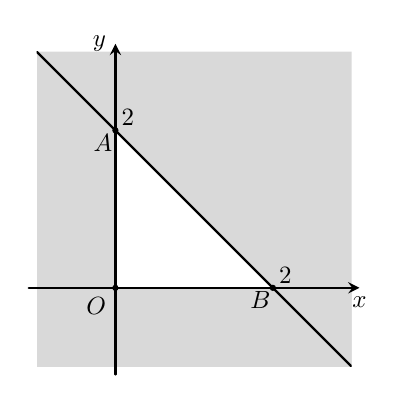
\begin{tikzpicture}[line join=round, line cap=round,>=stealth,thick]
			\tikzset{every node/.style={scale=0.9}}
			\begin{scope}
				\clip (-1,-1) rectangle (3,3);
				\fill[gray!30] (-1,-1) rectangle (0,3);
				\fill[gray!30] (-1,3)--(3,-1)--(3,3)--cycle;
				\fill[gray!30] (-1,-1) rectangle (3,0);
				\draw (-1,3)--(3,-1);
			\end{scope}
			\draw[->] (-1.1,0)--(3.1,0) node[below]{$x$};
			\draw[->] (0,-1.1)--(0,3.1) node[left]{$y$};
			\fill (0,0)circle(0.04) node[below left]{$O$};
			\fill (0,2)circle(0.04)node[shift={(-135:.25)}]{$A$};
			\fill (2,0)circle(0.04)node[shift={(-135:.25)}]{$B$};
			\path(0,2)node[shift={(45:.25)}]{$2$};
			\path(2,0)node[shift={(45:.25)}]{$2$};
		\end{tikzpicture}}
	\loigiai{
		Miền nghiệm của hệ nằm bên phải trục tung nên $x\ge0$;\\
		Miền nghiệm của hệ nằm phía trên trục hoành nên $y\ge0$;\\
		Miền nghiệm có chứa điểm $O(0;0)$ và $0+0<2$ nên miền tam giác $OAB$ trong hình vẽ là miền nghiệm của hệ $\heva{& x\ge 0\\ & y\ge 0\\ & x+y\le 2.}$
	}
\end{ex}

\begin{ex}%[BG12-3in1, Nguyễn Xuân Bảo-Phạm Ngọc Trung]%[0H4N2-1]
	Cho tam giác đều $ ABC $ có có cạnh bằng $30$. Gọi $G$ là trọng tâm  $\triangle ABC$. Tính $AG$.
	\choice
	{$ 10 $}
	{$ 15\sqrt{2}$}
	{$ 5\sqrt{3} $}
	{\True $10\sqrt{3}$}
	\loigiai{
		\begin{center}
			\begin{tikzpicture}[scale=1, font=\footnotesize, line join=round, line cap=round, >=stealth]
				\coordinate[label=left:$B$] (B) at (0,0);
				\coordinate[label=right:$C$] (C) at (5,0);
				\coordinate[shift=(60:5),label=above:$A$] (A) at (B);
				\coordinate[label=below:$I$] (I) at ($(B)!0.5!(C)$);
				\coordinate[label=left:$G$] (G) at ($(A)!2/3!(I)$);
				\draw (A)--(B)--(C)--cycle (A)--(I);
			\end{tikzpicture}
		\end{center}
		Ta có  $AI^2=BA^2+BI^2-2\cdot BA \cdot BI \cdot \cos B=30^2+15^2-2 \cdot 30 \cdot 15 \cdot \cos 60^{\circ}=675 \Rightarrow AI=15\sqrt{3}$.	\\
		Vì $G$ là trọng tâm tam giác $ABC$ nên $AG=\dfrac{2}{3}AI=10\sqrt{3}$.
	}

\end{ex}

\begin{ex}%[0H4N2-2]
	Cho $\triangle ABC$ có $a=4$, $c=5$, $\widehat{B}=150^\circ$. Tính diện tích tam giác $ABC$.
	\choice
	{$S=10$}
	{\True $S=5$}
	{$S=5\sqrt{3}$}
	{$S=10\sqrt{3}$}
	\loigiai{
		Ta có $S=\dfrac{1}{2}ac\sin B=\dfrac{1}{2}\cdot 4\cdot 5\sin 150^\circ=5$.
	}
\end{ex}

\begin{ex}%[0H4H2-1]%[Phạm Văn Long, DCT10-NTH-HK1]
	Cho tam giác $ABC$ có $BC=a$, $CA=b$, $AB=c$. Mệnh đề nào sau đây đúng?
	\choice
	{\True Nếu $b^2+c^2-a^2>0$ thì góc $A$ nhọn}
	{Nếu $b^2+c^2-a^2>0$ thì góc $A$ tù}
	{Nếu $b^2+c^2-a^2<0$ thì góc $A$ nhọn}
	{Nếu $b^2+c^2-a^2<0$ thì góc $A$ vuông}
	\loigiai{
		Áp dụng định lý Cô-sin ta có
		\[\cos A=\dfrac{b^2+c^2-a^2}{2bc}.\]
		Nếu $b^2+c^2-a^2>0$ thì $\cos A>0$  suy ra góc $A$ nhọn.\\
		Nếu $b^2+c^2-a^2<0$ thì $\cos A<0$  suy ra góc $A$ tù.
	}
\end{ex}

\begin{ex}%[N]%[Nguyễn Thắng]giảng 10 New - 4in1, Nguyễn Vân Trường]%[0H4H1-2]
	Cho  góc nhọn $\alpha$. Khẳng định nào sau đây là {\bf sai}?
	\choice
	{$\sin 2\alpha >  0$}
	{$\cot \alpha > 0 $}
	{\True $\cos 2\alpha > 0 $}
	{$\tan \alpha >0 $}
	\loigiai{
		Do $\alpha$ là hai góc nhọn nên $2\alpha$ là góc tù nên  $\cos 2\alpha <0$.
	}
\end{ex}

\begin{ex}%[0-HK1-KN-7-HaDong-HaNoi-2324]%[VN-MT-6, Đoàn Thị Lý]%[0H5N1-3]
	Cho hình bình hành $ABCD$. Khẳng định nào sau đây đúng?
	\choice
	{$\overrightarrow{AB}=\overrightarrow{AC}$}
	{$\overrightarrow{AB}=\overrightarrow{CD}$}
	{\True $\overrightarrow{AD}=\overrightarrow{BC}$}
	{$\overrightarrow{AC}=\overrightarrow{DB}$}
	\loigiai{
		Khẳng định đúng là $\overrightarrow{AD}=\overrightarrow{BC}$.
	}
\end{ex}

\begin{ex}%[0-HK1-CTST-4-2324]%[VN-MT-9, Phúc Hậu]%[ID]%[0H5N2-2]
	Cho ba điểm phân biệt $A$, $B$, $C$. Trong các khẳng định sau, khẳng định nào \textbf{sai}?
	\choice
	{$\overrightarrow{AB}+\overrightarrow{BC}=\overrightarrow{AC}$}
	{$\overrightarrow{AB}-\overrightarrow{AC}=\overrightarrow{CB}$}
	{$\overrightarrow{CA}+\overrightarrow{BC}=\overrightarrow{BA}$}
	{\True $\overrightarrow{CB}-\overrightarrow{CA}=\overrightarrow{BA}$}
	\loigiai{
		Ta có $\overrightarrow{CB}-\overrightarrow{CA}=\overrightarrow{AB}$.}
\end{ex}

\begin{ex}%[0H5H2-2]
	Cho hình bình hành $ABCD$. Mệnh đề nào sau đây đúng?
	\choice
	{$\overrightarrow{DA}+\overrightarrow{DB}+\overrightarrow{BA}=\overrightarrow0$}
	{\True $\overrightarrow{DA}-\overrightarrow{DB}+\overrightarrow{DC}=\overrightarrow0$}
	{$\overrightarrow{DA}-\overrightarrow{DB}+\overrightarrow{CD}=\overrightarrow0$}
	{$\overrightarrow{DA}-\overrightarrow{DB}+\overrightarrow{DA}=\overrightarrow0$}
	\loigiai{
		\immini{Từ hình vẽ bên, ta thấy\\ $\overrightarrow{DA}-\overrightarrow{DB}+\overrightarrow{DC}=\overrightarrow {BA}+\overrightarrow{DC}=\overrightarrow {BA}+\overrightarrow{AB}=\overrightarrow{0}$.}
		{\begin{tikzpicture}[line join=round, line cap=round,thick]
				\coordinate (A) at (1,3);
				\coordinate (B) at (6,3);
				\coordinate (D) at (0,0);
				\coordinate (C) at ($(B)+(D)-(A)$);
				\draw(A)--(B)--(C)--(D)--cycle;
				\foreach \i/\g in {A/90,B/90,C/-90,D/-90}{\draw[fill=black](\i) circle (1pt) ($(\i)+(\g:3mm)$) node[scale=1]{$\i$};}
			\end{tikzpicture}
		}
	}
\end{ex}

\begin{ex}%[0-HK1-CD-1-SoBacNinh-2324]%[VN-MT-6, Tống Văn Ký]%[0H5H3-2]
	\immini[thm]{Cho tam giác $ABC$ có $M$ là trung điểm $BC$. Mệnh đề nào sau đây \textbf{sai}?
		\choice[2]
		{\True $\overrightarrow{AB}-\overrightarrow{AC}=2\overrightarrow{BM}$}
		{$\overrightarrow{AB}+\overrightarrow{AC}=2\overrightarrow{AM}$}
		{$\overrightarrow{MB}+\overrightarrow{MC}=\overrightarrow0$}
		{$\overrightarrow{AC}-\overrightarrow{AB}=2\overrightarrow{BM}$}
	}{\begin{tikzpicture}[font=\footnotesize, line join=round, line cap=round, >=stealth, scale=1]
			\path
			(0:0) coordinate (B)++(0:3) coordinate (C)
			($(B)!1/2!(C)$) coordinate (M)
			(B)++(60:3) coordinate (A)
			;
			\draw
			(M)--(A)--(B)--(C)--(A)
			;
			\foreach \x/\g in {M/-90,C/0,A/90,B/180}
			\fill (\x) circle (1pt)
			+(\g:3mm) node{$\x$};
		\end{tikzpicture}
	}
	\loigiai{
		Ta có $\overrightarrow{AB}-\overrightarrow{AC} =\overrightarrow{CB}=2\overrightarrow{MB} =-2\overrightarrow{BM}$ nên khẳng định $\overrightarrow{AB}-\overrightarrow{AC} =2\overrightarrow{BM}$ là sai.
	}
\end{ex}

\begin{ex}%[0H5N4-1]
	%Câu 3 :
	Cho hai véc-tơ $\overrightarrow{a},\overrightarrow{b}$ khác véc-tơ-không thỏa mãn $\overrightarrow{a}\cdot \overrightarrow{b}=-\left| \overrightarrow{a} \right|\cdot \left| \overrightarrow{b} \right|$. Khi đó góc giữa hai véc-tơ $\overrightarrow{a},\overrightarrow{b}$ bằng
	\choice
	{$\left( \overrightarrow{a};\overrightarrow{b} \right)=45^{\circ}$}
	{$\left( \overrightarrow{a};\overrightarrow{b} \right)=0^{\circ}$}
	{\True $\left( \overrightarrow{a};\overrightarrow{b} \right)=180^{\circ}$}
	{$\left( \overrightarrow{a};\overrightarrow{b} \right)=90^{\circ}$}
	\loigiai{
		Ta có  $\overrightarrow{a}\cdot \overrightarrow{b}=-\left| \overrightarrow{a} \right|\cdot \left| \overrightarrow{b} \right|\Rightarrow \left| \overrightarrow{a} \right|\cdot \left| \overrightarrow{b} \right|\cdot \cos \left( \overrightarrow{a},\overrightarrow{b} \right)=-\left| \overrightarrow{a} \right|\cdot \left| \overrightarrow{b} \right|\Rightarrow \cos \left( \overrightarrow{a},\overrightarrow{b} \right)=-1\Rightarrow \left( \overrightarrow{a},\overrightarrow{b} \right)=180^\circ$.
	}
\end{ex}

\begin{ex}%[Mức 2]%[Dự án Giảng 10-11 Nhóm Toán & LaTex, Lê Minh Thiện Anh]%[0H5H4-2]
	Tam giác $ABC$ vuông ở $A$ và có $BC=2AC$. Tính $\cos\left(\overrightarrow{AC},\overrightarrow{CB}\right)$.
	\choice
	{$\cos\left(\overrightarrow{AC},\overrightarrow{CB}\right)=\dfrac{1}{2}$}
	{\True $\cos\left(\overrightarrow{AC},\overrightarrow{CB}\right)=-\dfrac{1}{2}$}
	{$\cos\left(\overrightarrow{AC},\overrightarrow{CB}\right)=\dfrac{\sqrt{3}}{2}$}
	{$\cos\left(\overrightarrow{AC},\overrightarrow{CB}\right)=-\dfrac{\sqrt{3}}{2}$}
	\loigiai{
		Xác định được $\left(\overrightarrow{AC},\overrightarrow{CB}\right)=180^\circ -\widehat{ACB}$.\\
		Ta có $ \cos \widehat{ACB}=\dfrac{AC}{BC}=\dfrac{1}{2} \Rightarrow \widehat{ACB}=60^\circ$.\\
		Vậy $\cos\left(\overrightarrow{AC},\overrightarrow{CB}\right)=\cos{120^\circ }=-\dfrac{1}{2}$.
	}
\end{ex}

\begin{ex} %[0D8N1-1]
	Có $3$ cây bút đỏ và $4$ cây bút xanh trong một hộp bút. Hỏi có bao nhiêu cách lấy ra một cây bút từ hộp bút?
	\choice
	{$4$}
	{$12$}
	{\True $7$}
	{$3$}
	\loigiai{
		Số cách chọn $1$ cây bút đỏ là $3$ cách.\\
		Số cách chọn $1$ cây bút xanh là $4$ cách.\\
		Vậy có $3+4=7$ cách chọn một cây bút.
	}
\end{ex}

\begin{ex}%[0D8H1-3]
	Từ tập $\{1;2;3;4;5;6\}$ lập được bao nhiêu số tự nhiên có nhiều nhất hai chữ số?
	\choice
	{$30$}
	{\True $42$}
	{$36$}
	{$6$}
	\loigiai
	{
		\begin{itemize}
			\item Số một chữ số có $6$ số.
			\item Số có hai chữ số có $6^2=36$ số.
		\end{itemize}
		Vậy có tất cả $36+6=42$ số thỏa mãn yêu cầu bài toán.
	}
\end{ex}

\begin{ex}%[BG - 10 New - 3in1, Nguyễn Văn Cường (Cường NV)]%[0D8H1-2]
	Một người có $4$ cái quần, $6$ cái áo, $3$ chiếc cà vạt. Để chọn mỗi thứ một món thì có bao nhiêu cách chọn bộ ``quần-áo-cà vạt'' khác nhau?
	\choice
	{$13$}
	{\True $72$}
	{$12$}
	{$30$}
	\loigiai{
		Để chọn một bộ ``quần-áo-cà vạt'', ta có
		\begin{itemize}
			\item Có $4$ cách chọn quần.
			\item Có $6$ cách chọn áo.
			\item Có $3$ cách chọn cà vạt.
		\end{itemize}
		Vậy theo qui tắc nhân ta có $4 \times 6 \times 3=72$ cách.
	}
\end{ex}

\begin{ex}%[0D8N2-1]
	Cho $k, n \in \mathbb{N}^*$ và $n \geq k$. Công thức nào dưới đây đúng?
	\choice
	{$\mathrm{C}_n^k=\dfrac{n !}{k !}$}
	{$\mathrm{C}_n^k=\dfrac{n !}{(n-k) !}$}
	{\True $\mathrm{C}_n^k=\dfrac{n !}{(n-k) ! k !}$}
	{$\mathrm{C}_n^k=n!$}
	\loigiai{
		Ta có $\mathrm{C}_n^k=\dfrac{n !}{(n-k) ! k !}$.
	}
\end{ex}

\begin{ex}%[0D8H2-3]%[Dự án đề kiểm tra Toán 10 CHKI NH23-24- lamnguyen]%[THPT - Đồng nai]
	Từ các chữ số $1,2,3,4,5$ có thể lập được bao nhiêu số tự nhiên có ba chữ số đôi một khác nhau?
	\choice
	{\True $60$}
	{$120$}
	{$3125$}
	{$24$}
	\loigiai{
		Mỗi cách lập số tự nhiên có ba chữ số đôi một khác nhau từ một tập có $5$ chữ số khác nhau và khác $0$ là một chỉnh hợp chập $3$ của $5$ phần tử.\\
		Vậy số các số lập được là $\mathrm{A}_5^3=60$ (số).
	}
\end{ex}

\begin{ex}%[0D8N3-2]%[HKII-NGUYỄN THÁI BÌNH 2324]%[TheHung Nguyen]
	Khai triển nhị thức $(x+3y)^4$ thu được kết quả là
	\choice
	{$x^4-4 x^3 y+18 x^2 y^2-36 x y^3+27 y^4$}
	{\True $x^4+12 x^3 y+54 x^2 y^2+108 x y^3+81 y^4$}
	{$x^4+4 x^3 y+18 x^2 y^2+36 x y^3+27 y^4$}
	{$x^4-12 x^3 y+54 x^2 y^2-108 x y^3+81 y^4$}
	\loigiai{
		Ta có $(x+3y)^4=x^4+12x^3y+54x^2y^2+108xy^3+81 y^4$.
	}
\end{ex}

\begin{ex}%[0D8H3-3]
	Hệ số của số hạng chứa $x^6y$ trong khai triển $\left(3x^2-y\right)^4$ là
	\choice
	{$-12$}
	{$54$}
	{\True $-108$}
	{$81$}
	\loigiai{
		Khai triển $\left(3x^2-y\right)^4$ ta được
		\begin{align*}
			\left(3x^2-y\right)^4 = & \, \left(3x^2\right)^4 + 4\left(3x^2\right)^3 (-y) + 6\left(3x^2\right)^2 (-y)^2 + 4\left(3x^2\right) (-y)^3 + (-y)^4 \\
			=                       & \, 81x^8 - 108x^6y + 54x^4y^2 - 12x^2y^3 + y^4.
		\end{align*}
		Hệ số của  $x^6y$ là  $-108$.
	}
\end{ex}

\begin{ex}%[Dự án Đề GK2 PNL Cấu Trúc 2025]%[Đào-V- Thuỷ]%[0H9N1-3]
	Trong mặt phẳng $Oxy$, cho điểm $A(1;-4)$, điểm $B(2;-1)$. Toạ độ véc-tơ $\vec{AB}$ là
	\choice
	{$\vec{AB}= (-1;-3)$}
	{$\vec{AB}= (3;-5)$}
	{\True $\vec{AB}= (1;3)$}
	{$\vec{AB}= (1;-3)$}
	\loigiai
	{
		Ta có $\vec{AB}= (2-1; -1+4)= (1;3)$.
	}
\end{ex}

\begin{ex}%[Dự án EX-10-11-Chuẩn hóa]%[Hoàng Thanh Phương]%[0H9H1-3]
	Trong hệ trục tọa độ $Oxy$, cho tam giác $ABC$ có $A(-4;1)$, $B(2;4)$. Tìm tọa độ điểm $C$ sao cho $G(2;-2)$ là trọng tâm của tam giác $ABC$.
	\choice
	{$C(8;11)$}
	{$C(12;11)$}
	{\True $C(8;-11)$}
	{$C(-8;-11)$}
	\loigiai{ Vì $G$ là trọng tâm tam giác $ABC$ nên
		\[ \heva{&x_G=\dfrac{x_A+x_B+x_C}{3}\\&y_G=\dfrac{y_A+y_B+y_C}{3}} \Leftrightarrow \heva{&x_C=3x_G-x_A-x_B=3 \cdot 2-(-4)-2=8\\&y_C=3y_G-y_A-y_B=3 \cdot (-2)-1-4=-11.} \]
		Suy ra $C(8;-11)$.}
\end{ex}

\begin{ex}%[0H9H1-4]
	Trong mặt phẳng tọa độ $Oxy$, cho hình thoi $ABCD$ có $A(-1;0)$, $B(-2;3)$, $C(1;2)$. Tọa độ đỉnh $D$ là
	\choice
	{$(-1;-2)$}
	{$(-2;1)$}
	{\True $(2;-1)$}
	{$(2;1)$}
	\loigiai{
		Vì $AB=\sqrt{(-1)^2+3^2}=\sqrt{10}$; $BC=\sqrt{3^2+(-1)^2}=\sqrt{10}$ nên tứ giác $ABCD$ là hình thoi khi tứ giác $ABCD$ là hình bình hành.\\
		$ABCD$ là hình bình hành khi $\vv{AB}=\vv{DC}\Leftrightarrow\heva{&1-x=-2+1\\&2-y=3-0}\Leftrightarrow\heva{&x=2\\&y=-1.}$
	}
\end{ex}

\begin{ex}%[0H9N2-1]
	%Câu 10 :
	Trong mặt phẳng tọa độ $Oxy$ cho ba điểm $A(1;2), B(-1;1)$ và $C(5;-1)$. Tính cosin của góc $\widehat{BAC}$.
	\choice
	{$\dfrac{1}{2}$}
	{$-\dfrac{2}{3}$}
	{$-\dfrac{2}{5}$}
	{\True $-\dfrac{\sqrt{5}}{5}$}
	\loigiai{
		\begin{eqnarray*}
			\widehat{BAC}&=&\left( \overrightarrow{AB},\overrightarrow{AC} \right),\;
			\overrightarrow{AB} = \left( -2;-1 \right),\; \overrightarrow{AC}=\left( 4;-3 \right). \\
			\cos A&=&\dfrac{\overrightarrow{AB}\cdot \overrightarrow{AC}}{\left| \overrightarrow{AB} \right|\cdot \left| \overrightarrow{AC} \right|}=\dfrac{-2\cdot 4+(-1)\cdot (-3)}{\sqrt{(-2)^2+(-1)^2}\cdot \sqrt{4^2}+(-3)^2}=-\dfrac{\sqrt{5}}{5}.
		\end{eqnarray*}

	}
\end{ex}
\begin{ex}
	Cho hai vectơ $\vec{u}=(x;y)$ và $\vec{v}=(x';y')$. Khi đó
	\choice
	{$\vec{u}+\vec{v}=(x+y;x'+y')$}
	{\True $\vec{u}+\vec{v}=(x+x';y+y')$}
	{$\vec{u}+\vec{v}=(x-y;x'-y')$}
	{$\vec{u}+\vec{v}=(xy;x'y')$}
\end{ex}
\begin{ex}%[Đề HK1 THPT Chuyên Võ Nguyên Giáp, Quảng Bình, 2022-2023]%[Nguyễn Trung Kiên, dự án 10EX-HK1-2223 đợt 2]%[0H9H2-2]
	Trong mặt phẳng $Oxy$, cho tam giác $ABC$ biết $A(1; 3)$, $B(-2;-2)$, $C(3; 1)$. Giá trị $\cos\widehat{BAC}$ bằng
	\choice
	{$\cos\widehat{BAC}=-\dfrac{1}{\sqrt{17}}$}
	{\True $\cos\widehat{BAC}=\dfrac{1}{\sqrt{17}}$}
	{$\cos\widehat{BAC}=\dfrac{2}{\sqrt{17}}$}
	{$\cos\widehat{BAC}=-\dfrac{2}{\sqrt{17}}$}
	\loigiai
	{Ta có $\overrightarrow{AB}=(-3;-5)$, $AB=\sqrt{(-3)^2+(-5)^2} = \sqrt{34}$, $\overrightarrow{AC}=(2;-2)$, $AC=\sqrt{2^2+(-2)^2}=2\sqrt{2}$ nên
		\[\cos\widehat{BAC}=\cos\left(\overrightarrow{AB},\overrightarrow{AC}\right) = \dfrac{\overrightarrow{AB}\cdot \overrightarrow{AC}}{AB\cdot AC} = \dfrac{-6+10}{\sqrt{34}\cdot 2\sqrt{2}} = \dfrac{1}{\sqrt{17}}.\]}
\end{ex}
\begin{ex}%[VN-MT-9]%[0-TK-HK1-KN-8-2425, Nguyễn Quang Hiệp]%[0H5H3-5]
	Cho tam giác $ABC$, gọi $M$ là điểm thuộc cạnh $BC$ sao cho $BM=3MC$. Khẳng định nào dưới đây đúng?
	\choice
	{\True $\overrightarrow{AM}=\dfrac{1}{4}\overrightarrow{AB}+\dfrac{3}{4}\overrightarrow{AC}$}
	{$\overrightarrow{AM}=\dfrac{2}{3}\overrightarrow{AB}+\dfrac{1}{3}\overrightarrow{AC}$}
	{$\overrightarrow{AM}=\dfrac{3}{4}\overrightarrow{AB}+\dfrac{1}{4}\overrightarrow{AC}$}
	{$\overrightarrow{AM}=\dfrac{5}{4}\overrightarrow{AB} - \dfrac{3}{4}\overrightarrow{AC}$}
	\loigiai{
		Ta có
		\begin{align*}
			\overrightarrow{AM}=\overrightarrow{AB}+\overrightarrow{BM}=\overrightarrow{AB}+\dfrac{3}{4}\overrightarrow{BC}.
		\end{align*}
		Mà $\overrightarrow{BC}=\overrightarrow{AC} - \overrightarrow{AB}$ nên
		\begin{align*}
			\overrightarrow{AM}=\overrightarrow{AB}+\dfrac{3}{4}\left(\overrightarrow{AC} - \overrightarrow{AB}\right)=\overrightarrow{AB}+\dfrac{3}{4}\overrightarrow{AC} - \dfrac{3}{4}\overrightarrow{AB}=\dfrac{1}{4}\overrightarrow{AB}+\dfrac{3}{4}\overrightarrow{AC}.
		\end{align*}
		Vậy đáp án đúng là $\overrightarrow{AM}=\dfrac{1}{4}\overrightarrow{AB}+\dfrac{3}{4}\overrightarrow{AC}$.
	}
\end{ex}

\begin{ex}
	Cho hình chữ nhật $ABCD$ có $AB=8$, $AD=5$. Tích $\vec{AB} \cdot \vec{BD}$.
	\choice
	{$\vec{AB} \cdot \vec{BD}=62$}
	{$\vec{AB} \cdot \vec{BD}=64$}
	{$\vec{AB} \cdot \vec{BD}=-62$}
	{$\vec{AB} \cdot \vec{BD}=-64$}
	\loigiai{
		Giả thiết không cho góc, ta phân tích các vectơ $\vec{AB}$, $\vec{BD}$ theo các vectơ có giá vuông góc với nhau.\\
		Ta có $\vec{AB} \cdot \vec{BD}=\vec{AB} \cdot \left(\vec{BA}+\vec{BC}\right)=\vec{AB} \cdot \vec{BA}+\vec{AB} \cdot \vec{BC}=-\vec{AB} \cdot \vec{AB}+0=-AB^2=-64$
	}
\end{ex}
\begin{ex}%[0-HK1-KN-2-NguyenTrai-HaNoi-23-24]%[VN-MT-6, Phạm Hoàng Điệp]%[0H9H1-4]
	Trong mặt phẳng tọa độ $ Oxy $, cho ba điểm $ A(2;-4) $, $ B(6;0) $, $ C(m;4) $. Tìm giá trị của $ m $ để ba điểm $ A $, $ B $, $ C $ thẳng hàng.
	\choice
	{$7$}
	{$8$}
	{$9$}
	{\True $10$}
	\loigiai{
		Ta có $ \overrightarrow{AB}=(4;4) $, $ \overrightarrow{AC}=(m-2;8) $.	\\
		Để $ 3 $ điểm $ A $, $ B $, $ C $ thẳng hàng thì
		\[\overrightarrow{AB} \, \text {cùng phương} \, \overrightarrow{AC} \Leftrightarrow \dfrac{m-2}{4}=\dfrac{8}{4}\Leftrightarrow m=10. \]
		Vậy $ m=10 $.
	}
\end{ex}

\TL

\begin{ex}%[De-chuan-hoa-so-13]%[Huỳnh Quy]%[0H4H2-1]
	Cho tam giác $ABC$ có $AB=2$, $AC=4$, $\widehat{A}=60^\circ$. Tính độ dài cạnh $BC$.
	\loigiai{
		Áp dụng định lý cô-sin cho tam giác $ABC$ ta có
		\begin{eqnarray*}
			BC^2&=&AB^2+AC^2-2\cdot AB\cdot AC\cdot \cos A\\
			&=& 2^2+4^2-2\cdot 2\cdot 4\cdot \cos 60^\circ\\
			&=&12.
		\end{eqnarray*}
		Vậy $BC=2\sqrt{3}$.
	}
\end{ex}

\begin{ex}
	Khai triển nhị thức Newton $\left(3x-\dfrac12y \right)^5$.
	\loigiai{
		\begin{align*}
			\left(3x-\dfrac12y \right)^5&=\mathrm{C}_5^0\left(3x\right)^5+\mathrm{C}_5^1\left(3x\right)^4\left(-\dfrac12y\right)^1+ \mathrm{C}_5^2\left(3x\right)^3\left(-\dfrac12y\right)^2 + \mathrm{C}_5^3\left(3x\right)^2\left(-\dfrac12y\right)^3 +\mathrm{C}_5^4\left(3x\right)^1\left(-\dfrac12y\right)^4 +\mathrm{C}_5^5\left(-\dfrac12y\right)^5\\
			&= 3^5x^5-\dfrac52\cdot 3^4x^4y+\dfrac{15}{4}\cdot 3^3x^3y^2-\dfrac{15}{8}\cdot 3^2x^2y^3+\dfrac{5}{16}\cdot 3xy^4-\dfrac{1}{32}y^5 \\
			&= 243x^5-\dfrac{405}{2}x^4y+\dfrac{405}{4}x^3y^2-\dfrac{135}{4}x^2y^3+\dfrac{15}{16}xy^4-\dfrac{1}{32}y^5.
		\end{align*}
	}
\end{ex}

\begin{ex}%[0D8V2-6]%[Dự án đề kiểm tra Toán 10 GHKI NH23-24- Nguyễn Hữu Duy]%[SGD Bắc Ninh]
	Cho lưới ô vuông gồm $5 \times 6$ hình vuông đơn vị. Gọi $A$ là điểm nằm ở góc trái dưới và $B$ là điểm nằm ở góc phải trên của lưới ô vuông (như hình vẽ). Để đi từ điểm $A$ đến điểm $B$	trên lưới ô vuông, một con kiến di chuyển ngẫu nhiên sang phải hoặc lên trên theo các đoạn thẳng là các cạnh của các hình vuông đơn vị. Hỏi con kiến có bao nhiêu cách để đi từ $A$ đến $B$?
	\begin{center}
		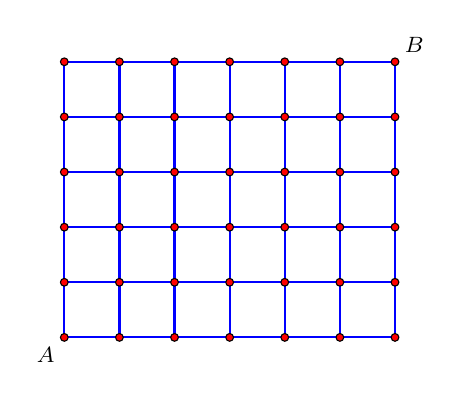
\begin{tikzpicture}[scale=.7, font=\footnotesize,line join=round, line cap=round, >=stealth]
			\path (0,0) coordinate (A) node[below left]{$A$}
			(6,5) coordinate (B) node[above right]{$B$}
			;
			\draw[step=1,blue,thick] (A) grid (B);
			%			\foreach \x/\g in {A/-120,B/60} \draw[fill = red] (\x) circle (2pt)+(\g:4mm)node{$\x$};
			\draw[step=1,blue,thick] (A) grid (B);
			\foreach \i in {0,1,2,3,4,5,6} {
					\foreach \j in {0,1,2,3,4,5} {
							\draw[fill = red] (\i,\j) circle (2pt);
						}
				}
		\end{tikzpicture}
	\end{center}
	\loigiai{
		Ta coi mỗi lần di chuyển qua một đoạn thẳng đơn vị là một “bước”. Muốn đi từ $A$ đến $B$ con kiến phải đi $11$ “bước”, gồm $5$ “bước” từ dưới lên trên và $6$ “bước” từ trái sang phải.\\
		Có $\mathrm{C}_{11}^5$ cách chọn $5$ “bước” từ dưới lên trên trong tổng số $11$ “bước”, còn $6$ “bước” còn lại con kiến sẽ “bước” từ trái sang phải. Vậy, con kiến có $\mathrm{C}_{11}^5 = 462$ cách đi từ $A$ đến $B$.
	}
\end{ex}

\begin{ex}%[0H5C4-7]%[CTST - Lớp 10 - Ôn tập cuối học kì 1 - Đề 4]%[Phạm Văn Long]
	Một chất điểm ở vị trí điểm $O$ chịu tác động bởi ba lực $\vec{F}_1, \vec{F}_2, \vec{F}_3$ có độ lớn là $F_1=6$N, $F_2=4$N, $F_3=2\sqrt{5}$N, góc tạo bởi hai lực $\vec{F}_1$ và $\vec{F}_3$ là $\alpha=60^{\circ}$ (tham khảo hình vẽ). Hỏi chất điểm trên phải chịu tác động hợp lực có độ lớn là bao nhiêu Newton N? (làm tròn đến hàng phần trăm).
	\begin{center}
		\begin{tikzpicture}[=>stealth,line join=round,line cap=round,thick, font=\footnotesize, scale=.9]
			\path
			(0,0)node[above]{$\vec{F}_2$}coordinate (F2)
			(8,0)node[above]{$\vec{F}_1$}coordinate (F1)
			(5,-3)node[left]{$\vec{F}_3$}coordinate (F3);
			\coordinate (O) at ($(F2)!0.4!(F1)$);
			\draw[red,->] (O)--(F2);
			\draw[->] (O)--(F1);
			\draw[blue,->] (O)--(F3);
			\fill[red,black] (O)node[above]{$O$} circle (1pt);
		\end{tikzpicture}
	\end{center}
	% \shortans{5,74}
	%Hình vẽ
	\loigiai{
		\begin{center}
			\begin{tikzpicture}[=>stealth,line join=round,line cap=round,thick, font=\footnotesize, scale=1.0]
				\path
				(0,0)node[above]{$\vec{F}_2$}coordinate (F2)
				(8,0)node[above]{$\vec{F}_1$}coordinate (F1)
				(5,-3)node[above left]{$\vec{F}_3$}coordinate (F3)
				(3.2,-3)node[below]{$F$} coordinate (F)
				(5,-3)node[below]{$C$};
				\coordinate (O) at ($(F2)!0.4!(F1)$);
				\path
				(F3)++(0:4.8)coordinate (B)node[below]{$B$}
				(B)++(0:-3.2)coordinate (E)node[below]{$E$}
				(F3)++(90:3)coordinate (G)node[above]{$G$};
				\draw (B)node[right]{$\vec{F}_1+\vec{F}_3$} (F1)node[right]{$A$} (F2)node[left]{$D$};
				\draw[red,->] (O)--(F2);
				\draw[->] (O)--(F1);
				\draw[blue,->] (O)--(F3);
				\draw[->] (O)--(E);
				\draw[dashed] (F3)--(B)--(F1) (O)--(B) (O)--(F)--(F3) (F2)--(E) (F3)--(G);
				\fill[black] (O)node[above]{$O$} circle (1.2pt) (F)circle (1.2pt) (F3)circle (1.2pt) (B)circle (1.2pt) (F1)circle (1.2pt) (F2)circle (1.2pt) (G)circle (1.2pt) (E)circle (1.2pt);
			\end{tikzpicture}
		\end{center}
		Ta dựng hình bình hành $OABC$, suy ra $\overrightarrow{OB}=\vec{F}_1+\vec{F}_3$.\\
		Tương tự, ta dựng hình bình hành $ODEB$, suy ra $\overrightarrow{OE}=\vec{F}_1+\vec{F}_2+\vec{F}_3$.\\
		Hợp lực tác động lên chất điểm $O$ là độ lớn của vectơ $\overrightarrow{OE}$.\\
		Dựng tam giác $O G C$ vuông tại $G$, ta có
		\[\cos \alpha=\dfrac{O G}{O C} \Rightarrow O G=O C \cdot \cos \alpha=\sqrt{5}.\]
		Suy ra $F C=O G=\sqrt{5}$.\\
		Ta có $C E=C B-E B=O A-O D=2, E F=F C+C E=\sqrt{5}+2$.\\
		Khi đó $O F=\sqrt{O C^2-F C^2}=\sqrt{(2 \sqrt{5})^2-(\sqrt{5})^2}=\sqrt{15}$.\\
		Do đó, $O E=\sqrt{O F^2+F E^2}=\sqrt{15+(2+\sqrt{5})^2}=\sqrt{24+4 \sqrt{5}} \approx 5{,}74$.\\
		Vậy, vật chịu tác động một hợp lực có độ lớn là $5{,}74$(N).
	}
\end{ex}

\begin{ex}%[0H9V1-3]
	\immini{Một vật đồng thời bị ba lực tác động: lực tác động thức nhất $\overrightarrow{F_1}$ có độ lớn là $15$ N, lực tác động thức hai $\overrightarrow{F_2}$ có độ lớn là $12$ N, lực tác động thức ba $\overrightarrow{F_3}$ có độ lớn là $8$ N. Các lực này được biểu diễn bằng các véc-tơ như hình bên, với $\left(\overrightarrow{F_1},\overrightarrow{F_2}\right)=30^\circ$, $\left(\overrightarrow{F_1},\overrightarrow{F_3}\right)=45^\circ$  $\left(\overrightarrow{F_2},\overrightarrow{F_3}\right)=75^\circ$. Tính độ lớn lực tổng hợp tác động lên vật (làm tròn kết quả đến hàng đơn vị). }{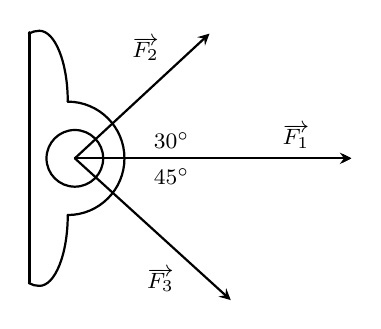
\begin{tikzpicture}[scale=0.9,font=\footnotesize,line join=round, line cap=round,>=stealth]
			\def\a{0.8}
			\def\b{1}
			%Vẽ các vật
			\draw[thick] (0:\a) arc (90:-90:{\a});
			\draw[thick] (0:\a) arc (0:90:{\a-0.4 and {\b} });
			\draw[thick] (-63.434:2.236*\a) arc (0:-90:{\a-0.4} and {\b});
			\draw [thick] (\a-\b+1.1,-\a) circle (\a-0.4);
			\draw [thick] (\a-\b+0.6,\b)  arc (90:120:{\a-0.5});
			\draw [thick] (\a-\b+0.6,-2*\a-\b)  arc (-90:-120:{\a-0.5});
			\draw [thick]  (\a-\b+0.46,-2*\a-\b+0.05)--(\a-\b+0.46,2*\a-0.62);
			%Vẽ các mũi tên
			\draw[->](\a-\b+1.1,-\a)--(4.8,-\a) node[above,pos=0.35]{$30^\circ$};
			\draw[->](\a-\b+1.1,-\a)--(4.8,-\a) node[above,pos=0.8, thick]{$\overrightarrow{F_1}$};
			\draw[->,thick](\a-\b+1.1,-\a)--(4.8,-\a) node[below,pos=0.35]{$45^\circ$};
			\draw[->, thick](\a-\b+1.1,-\a)--(2.8,1.2*\a) node[above left,pos=0.7]{$\overrightarrow{F_2}$};
			\draw[->, thick](\a-\b+1.1,-\a)--(3.1,-\a-2) node[below left,pos=0.7]{$\overrightarrow{F_3}$};
		\end{tikzpicture}}
	% \shortans{$26$ N}
	\loigiai{\immini{Chọn hệ trục tọa độ $Oxy$ như hình bên, $x$ và $y$ tính bằng Newton.\\
			Ta có $\overrightarrow{F_1}=(15;0)$.\\
			Vì $\left(\overrightarrow{F_1};\overrightarrow{F_2}\right)=30^\circ$ nên tọa độ $\overrightarrow{F_2}$ là \[\overrightarrow{F_2}=\left(12 \cos 30^\circ; 12 \sin 30^\circ \right)=(6 \sqrt{3};6).\]
			Vì $\left(\overrightarrow{F_1};\overrightarrow{F_3}\right)=45^\circ$ nên tọa độ $\overrightarrow{F_3}$ là \[\overrightarrow{F_3}=\left(8 \cos 45^\circ; -8 \sin 45^\circ \right)=(4 \sqrt{2};-4\sqrt{2}).\]}
		{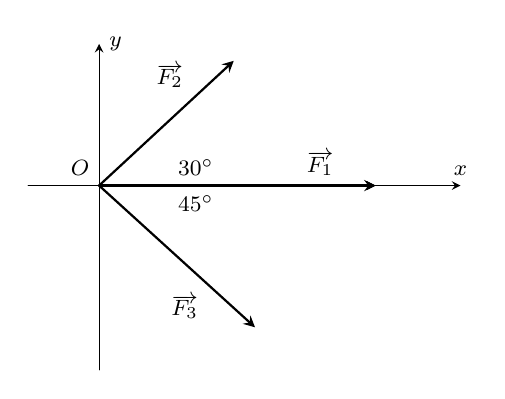
\begin{tikzpicture}[scale=0.9,font=\footnotesize,line join=round, line cap=round,>=stealth]
				\def\a{0.8}
				\def\b{1}
				%Vẽ trục tọa độ
				\draw[->](\a-\b+1.1-1,-\a)--(6,-\a) node[above, thick]{$x$};
				\draw[->](\a-\b+1.1,-\a-2.6)--(\a-\b+1.1,-\a+2) node[right, thick]{$y$};
				\draw (\a-\b+1.1,-\a) node [above left]{$O$};
				%Vẽ các mũi tên
				\draw[->](\a-\b+1.1,-\a)--(4.8,-\a) node[above,pos=0.35]{$30^\circ$};
				\draw[->](\a-\b+1.1,-\a)--(4.8,-\a) node[above,pos=0.8, thick]{$\overrightarrow{F_1}$};
				\draw[->,thick](\a-\b+1.1,-\a)--(4.8,-\a) node[below,pos=0.35]{$45^\circ$};
				\draw[->, thick](\a-\b+1.1,-\a)--(2.8,1.2*\a) node[above left,pos=0.7]{$\overrightarrow{F_2}$};
				\draw[->, thick](\a-\b+1.1,-\a)--(3.1,-\a-2) node[below left,pos=0.7]{$\overrightarrow{F_3}$};
			\end{tikzpicture}}
		Do đó, lực $\overrightarrow{F}$ tổng hợp các lực tác động lên vật có tọa độ là
		\[\overline{F}=\overrightarrow{F_1}+\overrightarrow{F_2}+\overrightarrow{F_3}=(15+6\sqrt{3}+4\sqrt{2};6-4\sqrt{2}).\]
		Độ lớn lực $\overrightarrow{F}$ tác động lên vật là
		\[\left| \overrightarrow{F} \right| = \sqrt{\left(15+6\sqrt{3}+4\sqrt{2}\right)^2+\left(6-4\sqrt{2}\right)^2} \approx 31 \; \text{N}.\]
		Vậy lực tổng hợp tác động lên vật có độ lớn khoảng là $31$ N.}
\end{ex}
\Closesolutionfile{ans}

